\documentclass{article}

\usepackage{fancyhdr}
\usepackage{lastpage}
\usepackage{extramarks}
\usepackage[usenames,dvipsnames]{color}
\usepackage{amsmath}
\usepackage{amsthm}
\usepackage{amsfonts}
\usepackage{tikz}

\usetikzlibrary{automata,positioning,calc}

\topmargin=-0.45in
\evensidemargin=0in
\oddsidemargin=0in
\textwidth=6.5in
\textheight=9.0in
\headsep=0.25in

\linespread{1.1}

\pagestyle{fancy}
\lhead{\hmwkAuthorName}
\chead{\hmwkClass\ (\hmwkClassInstructor\ \hmwkClassTime): \hmwkTitle}
\rhead{\firstxmark}
\lfoot{\lastxmark}
\cfoot{}
\renewcommand\headrulewidth{0.4pt}
\renewcommand\footrulewidth{0.4pt}

\setlength\parindent{0pt}

\newcommand{\enterProblemHeader}[1]{
    \nobreak\extramarks{#1}{#1 continued on next page\ldots}\nobreak
    \nobreak\extramarks{#1 (continued)}{#1 continued on next page\ldots}\nobreak
}

\newcommand{\exitProblemHeader}[1]{
    \nobreak\extramarks{#1 (continued)}{#1 continued on next page\ldots}\nobreak
    \nobreak\extramarks{#1}{}\nobreak
}

\setcounter{secnumdepth}{0}
\newcounter{homeworkProblemCounter}

\newcommand{\homeworkProblemName}{}
\newenvironment{homeworkProblem}[1][Problem \arabic{homeworkProblemCounter}]{
    \stepcounter{homeworkProblemCounter}
    \renewcommand{\homeworkProblemName}{#1}
    \section{\homeworkProblemName}
    \enterProblemHeader{\homeworkProblemName}
}{
    \exitProblemHeader{\homeworkProblemName}
}

\newcommand{\problemAnswer}[1]{
\noindent\framebox[\columnwidth][c]{\begin{minipage}{0.98\columnwidth}#1\end{minipage}}
}

\newcommand{\homeworkSectionName}{}
\newenvironment{homeworkSection}[1]{
    \renewcommand{\homeworkSectionName}{#1}
    \subsection{\homeworkSectionName}
    \enterProblemHeader{\homeworkProblemName\ [\homeworkSectionName]}
}{
    \enterProblemHeader{\homeworkProblemName}
}

\newcommand{\hmwkTitle}{Homework\ \#5}
\newcommand{\hmwkDueDate}{March 07, 2013 at 11:59pm}
\newcommand{\hmwkClass}{CS331}
\newcommand{\hmwkClassTime}{9:00am}
\newcommand{\hmwkClassInstructor}{Professor Zhang}
\newcommand{\hmwkAuthorName}{Josh Davis}

\title{
    \vspace{2in}
    \textmd{\textbf{\hmwkClass:\ \hmwkTitle}}\\
    \normalsize\vspace{0.1in}\small{Due\ on\ \hmwkDueDate}\\
    \vspace{0.1in}\large{\textit{\hmwkClassInstructor\ \hmwkClassTime}}
    \vspace{3in}
}

\author{\textbf{\hmwkAuthorName}}
\date{}

\begin{document}

\maketitle

\pagebreak

\begin{homeworkProblem}
    Let \(\Sigma = \{0, 1\}\). Consider the following language over \(\Sigma\),
    \( L = \{w \in \Sigma^* : w \mbox{ contains twice as many 0's as 1's }\} \)
    \\

    \textbf{Part One} Describe in pseudo-code a Turing machine, \(M\) that recognizes \(L\).
    \\

    The pseudo-code that describes \(M\) is as follows:

    \(M = \)`` On input string \(w\):
    \begin{enumerate}
        \item Start on the left side of the word, if the word is empty, move to \(q_{accept}\)
        \item Move to the left of the word
        \item Move right until we find a 1, cross it out. If we reach the end of the tape, move to stage 8
        \item Move back to the left of the word
        \item Scan right until the first 0 is found, cross it out. If we reach the end of the tape, move to \(q_{reject}\)
        \item Move back to the left of the word
        \item Scan right again until the second 0 is found, cross it out and move to stage 2. If we reach the end of the tape, move to \(q_{reject}\)
        \item Move to the left of the word
        \item Scan over the word, if we reach anything but an x, (0, 1), move to \(q_{reject}\), if we reach the end of the word, move to \(q_{accept}\)
    \end{enumerate}

    \textbf{Part Two} Formally define \(M\), where \(M = \langle \Sigma, \Gamma, Q, q_0, q_{accept}, q_{reject} \rangle\)
    \\

    \(M\) can be formally defined as follows:
    \begin{enumerate}
        \item \(\Gamma = \Sigma \cup \{\textvisiblespace, x\}\)
        \item \(Q = \{q_0, q_1, q_2, q_3, q_4, q_5, q_6, q_7, q_8, q_{accept}, q_{reject}\}\), the states
        \item \(q_0\), the start state
        \item Then \(\delta\) as given by the table:
            \begin{table}[ht]
                \centering
                \begin{tabular}{c || c | c | c | c}
                    \(\delta\) & 0 & 1 & x & \textvisiblespace \\
                    \hline
                    \(q_0\) & \((q_1, 0, L)\) & \((q_1, 1, L)\) & \((q_1, x, L)\) & \((q_{accept}, \textvisiblespace, L)\) \\
                    \(q_1\) & \((q_1, 0, L)\) & \((q_1, 1, L)\) & \((q_1, x, L)\) & \((q_2, \textvisiblespace, R)\) \\
                    \(q_2\) & \((q_2, 0, R)\) & \((q_3, x, L)\) & \((q_2, x, R)\) & \((q_7, \textvisiblespace, L)\) \\
                    \(q_3\) & \((q_3, 0, L)\) & \((q_3, 1, L)\) & \((q_3, x, L)\) & \((q_4, \textvisiblespace, R)\) \\
                    \(q_4\) & \((q_5, x, L)\) & \((q_4, 1, R)\) & \((q_4, x, R)\) & \((q_{reject}, \textvisiblespace, L)\) \\
                    \(q_5\) & \((q_5, 0, L)\) & \((q_5, 1, L)\) & \((q_5, x, L)\) & \((q_6, \textvisiblespace, R)\) \\
                    \(q_6\) & \((q_1, x, L)\) & \((q_6, 1, R)\) & \((q_6, x, R)\) & \((q_{reject}, \textvisiblespace, L)\) \\
                    \(q_7\) & \((q_7, 0, L)\) & \((q_7, 1, L)\) & \((q_7, x, L)\) & \((q_8, \textvisiblespace, L)\) \\
                    \(q_8\) & \((q_{reject}, 0, R)\) & \((q_{reject}, 1, R)\) & \((q_8, x, R)\) & \((q_{accept}, \textvisiblespace, L)\) \\
                \end{tabular}
            \end{table}
    \end{enumerate}

\end{homeworkProblem}

\pagebreak

\begin{homeworkProblem}
    Let \(\Sigma = \{0, 1\}\) and \(\Gamma = \{0, 1, \textvisiblespace, \#, x\}\). Write a Turing machine, \(M\),
    such that given any input \(w \in \Sigma^*\), \(M\) halts with tape content \(w\#w^R\).
    \\

    \textbf{Part One} Describe \(M\) in pseudo-code.
    \\

    The pseudo-code that describes \(M\) is as follows:

    \(M = \)`` On input string \(w\):
    \begin{enumerate}
        \item Start on the left side the word, write \# at the end and move left, go to the next stage
        \item If the head is on a 0, write an x and go to stage 3, if the head is on a 1 write an x and
            go to stage 5, if the head is on white space, go to \(q_{halt}\)
        \item Move to the right until we hit empty tape, write 0 and move left, go to next stage
        \item Move to the left until we hit an x, write a 0 and move left, go to stage 2
        \item Move to the right until we hit empty tape, write a 1 and move left, go to next stage
        \item Move to the left until we hit an x, write a 1 and move left, go to stage 2
    \end{enumerate}

    \textbf{Part Two} Formally define \(M\), where \(M = \langle \Sigma, \Gamma, Q, q_0, q_{accept}, q_{reject} \rangle\)
    \\

    \(M\) can be formally defined as follows:
    \begin{enumerate}
        \item \(\Gamma = \Sigma \cup \{\textvisiblespace, x, \#\}\)
        \item \(Q = \{q_0, q_1, q_2, q_3, q_4, q_5, q_6, q_7, q_8, q_{accept}, q_{reject}\}\), the states
        \item \(q_0\), the start state
        \item Then \(\delta\) as given by the table:
            \begin{table}[ht]
                \centering
                \begin{tabular}{c || c | c | c | c | c}
                    \(\delta\) & 0 & 1 & x & \# & \textvisiblespace \\
                    \hline
                    \(q_0\) & \((q_0, 0, R)\) & \((q_0, 1, R)\) & - & - & \((q_1, \#, L)\) \\
                    \(q_1\) & \((q_2, x, R)\) & \((q_4, x, R)\) & - & - & \((q_{halt}, \textvisiblespace, R)\) \\
                    \(q_2\) & \((q_2, 0, R)\) & \((q_2, 1, R)\) & - & \((q_2, \#, R)\) & \((q_3, 0, L)\) \\
                    \(q_3\) & \((q_3, 0, L)\) & \((q_3, 1, L)\) & \((q_1, 0, L)\) & \((q_3, \#, L)\) & - \\
                    \(q_4\) & \((q_4, 0, R)\) & \((q_4, 0, R)\) & - & \((q_4, \#, R)\) & \((q_5, 1, L)\) \\
                    \(q_5\) & \((q_5, 0, L)\) & \((q_5, 1, L)\) & \((q_1, 1, L)\) & \((q_5, \#, L)\) & \\
                \end{tabular}
            \end{table}
            \\
            Places with a - denote that the given configuration \textit{should} never be reached.
    \end{enumerate}
\end{homeworkProblem}

\pagebreak

\begin{homeworkProblem}
    Let \(M = \langle \Sigma, \Gamma, Q, q_0, \delta, q_{accept}, q_{reject}
    \rangle \) be a Turing machine where \(\Sigma = \{0, 1\}\), \(\Gamma = \{0, 1, \textvisiblespace \}\),

    \(Q = \{q_0, q_1, q_2, q_3, q_{accept}, q_{reject}\}\) and \(\delta\) is represented by the
    following table:

    \begin{table}[ht]
        \centering
        \begin{tabular}{c || c | c | c | c}
            \(\delta\) & 0 & 1 & \textvisiblespace \\
            \hline
            \(q_0\) & \((q_0, 0, R)\) & \((q_0, 1, R)\) & \((q_1, \textvisiblespace, L)\) \\
            \(q_1\) & \((q_2, 1, L)\) & \((q_1, 0, L)\) & \((q_3, 1, L)\) \\
            \(q_2\) & \((q_2, 0, L)\) & \((q_1, 1, L)\) & \((q_{accept}, \textvisiblespace, R)\) \\
            \(q_3\) & - & - & \((q_{accept}, \textvisiblespace, R)\) \\
        \end{tabular}
    \end{table}

    \textbf{Part One} Show the sequence of computation of \(M\) when given 01101 input.
    \\

    Read from left to right, top to bottom, the sequence is as follows:
    \begin{figure}[h]
        \centering
        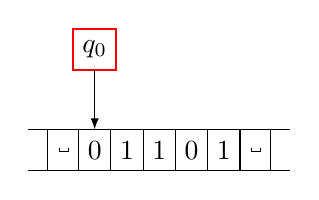
\begin{tikzpicture}[every node/.style={block}, block/.style={minimum height=1.5em,outer sep=0pt,draw,rectangle,node distance=0pt}]
            \node (C) {$1$};
            \node (B) [left=of C] {$1$};
            \node (A) [left=of B] {$0$};
            \node (0) [left=of A] {$\textvisiblespace$};
            \node (D) [right=of C] {$0$};
            \node (E) [right=of D] {$1$};
            \node (1) [right=of E] {$\textvisiblespace$};
            \node (F) [above = 0.75cm of A,draw=red,thick] {$q_0$};
            \draw[-latex] (F) -- (A);
            \draw (0.north west) -- ++(-.25cm,0) (0.south west) -- ++ (-.25cm,0) 
                (1.north east) -- ++(.25cm,0) (1.south east) -- ++ (.25cm,0);
        \end{tikzpicture}
        \hspace{20px}
        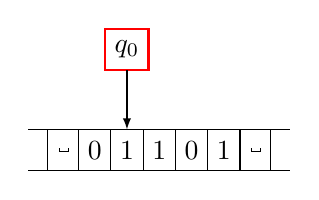
\begin{tikzpicture}[every node/.style={block}, block/.style={minimum height=1.5em,outer sep=0pt,draw,rectangle,node distance=0pt}]
            \node (C) {$1$};
            \node (B) [left=of C] {$1$};
            \node (A) [left=of B] {$0$};
            \node (0) [left=of A] {$\textvisiblespace$};
            \node (D) [right=of C] {$0$};
            \node (E) [right=of D] {$1$};
            \node (1) [right=of E] {$\textvisiblespace$};
            \node (F) [above = 0.75cm of B,draw=red,thick] {$q_0$};
            \draw[-latex] (F) -- (B);
            \draw (0.north west) -- ++(-.25cm,0) (0.south west) -- ++ (-.25cm,0) 
                (1.north east) -- ++(.25cm,0) (1.south east) -- ++ (.25cm,0);
        \end{tikzpicture}
        \hspace{20px}
        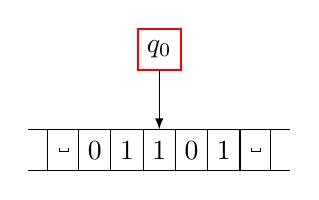
\begin{tikzpicture}[every node/.style={block}, block/.style={minimum height=1.5em,outer sep=0pt,draw,rectangle,node distance=0pt}]
            \node (C) {$1$};
            \node (B) [left=of C] {$1$};
            \node (A) [left=of B] {$0$};
            \node (0) [left=of A] {$\textvisiblespace$};
            \node (D) [right=of C] {$0$};
            \node (E) [right=of D] {$1$};
            \node (1) [right=of E] {$\textvisiblespace$};
            \node (F) [above = 0.75cm of C,draw=red,thick] {$q_0$};
            \draw[-latex] (F) -- (C);
            \draw (0.north west) -- ++(-.25cm,0) (0.south west) -- ++ (-.25cm,0) 
                (1.north east) -- ++(.25cm,0) (1.south east) -- ++ (.25cm,0);
        \end{tikzpicture}
        \hspace{20px}
        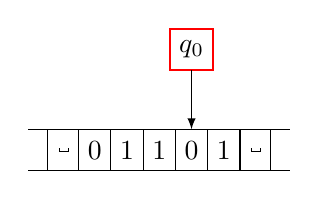
\begin{tikzpicture}[every node/.style={block}, block/.style={minimum height=1.5em,outer sep=0pt,draw,rectangle,node distance=0pt}]
            \node (C) {$1$};
            \node (B) [left=of C] {$1$};
            \node (A) [left=of B] {$0$};
            \node (0) [left=of A] {$\textvisiblespace$};
            \node (D) [right=of C] {$0$};
            \node (E) [right=of D] {$1$};
            \node (1) [right=of E] {$\textvisiblespace$};
            \node (F) [above = 0.75cm of D,draw=red,thick] {$q_0$};
            \draw[-latex] (F) -- (D);
            \draw (0.north west) -- ++(-.25cm,0) (0.south west) -- ++ (-.25cm,0) 
                (1.north east) -- ++(.25cm,0) (1.south east) -- ++ (.25cm,0);
        \end{tikzpicture}

        \vspace{20px}

        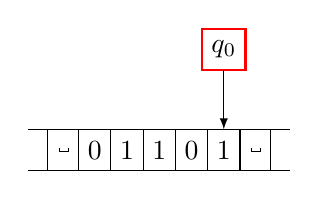
\begin{tikzpicture}[every node/.style={block}, block/.style={minimum height=1.5em,outer sep=0pt,draw,rectangle,node distance=0pt}]
            \node (C) {$1$};
            \node (B) [left=of C] {$1$};
            \node (A) [left=of B] {$0$};
            \node (0) [left=of A] {$\textvisiblespace$};
            \node (D) [right=of C] {$0$};
            \node (E) [right=of D] {$1$};
            \node (1) [right=of E] {$\textvisiblespace$};
            \node (F) [above = 0.75cm of E,draw=red,thick] {$q_0$};
            \draw[-latex] (F) -- (E);
            \draw (0.north west) -- ++(-.25cm,0) (0.south west) -- ++ (-.25cm,0) 
                (1.north east) -- ++(.25cm,0) (1.south east) -- ++ (.25cm,0);
        \end{tikzpicture}
        \hspace{20px}
        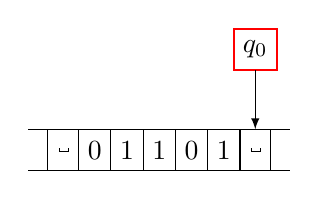
\begin{tikzpicture}[every node/.style={block}, block/.style={minimum height=1.5em,outer sep=0pt,draw,rectangle,node distance=0pt}]
            \node (C) {$1$};
            \node (B) [left=of C] {$1$};
            \node (A) [left=of B] {$0$};
            \node (0) [left=of A] {$\textvisiblespace$};
            \node (D) [right=of C] {$0$};
            \node (E) [right=of D] {$1$};
            \node (1) [right=of E] {$\textvisiblespace$};
            \node (F) [above = 0.75cm of 1,draw=red,thick] {$q_0$};
            \draw[-latex] (F) -- (1);
            \draw (0.north west) -- ++(-.25cm,0) (0.south west) -- ++ (-.25cm,0) 
                (1.north east) -- ++(.25cm,0) (1.south east) -- ++ (.25cm,0);
        \end{tikzpicture}
        \hspace{20px}
        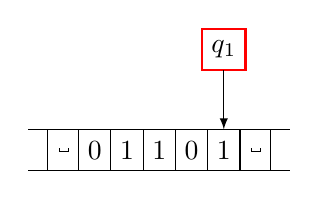
\begin{tikzpicture}[every node/.style={block}, block/.style={minimum height=1.5em,outer sep=0pt,draw,rectangle,node distance=0pt}]
            \node (C) {$1$};
            \node (B) [left=of C] {$1$};
            \node (A) [left=of B] {$0$};
            \node (0) [left=of A] {$\textvisiblespace$};
            \node (D) [right=of C] {$0$};
            \node (E) [right=of D] {$1$};
            \node (1) [right=of E] {$\textvisiblespace$};
            \node (F) [above = 0.75cm of E,draw=red,thick] {$q_1$};
            \draw[-latex] (F) -- (E);
            \draw (0.north west) -- ++(-.25cm,0) (0.south west) -- ++ (-.25cm,0) 
                (1.north east) -- ++(.25cm,0) (1.south east) -- ++ (.25cm,0);
        \end{tikzpicture}
        \hspace{20px}
        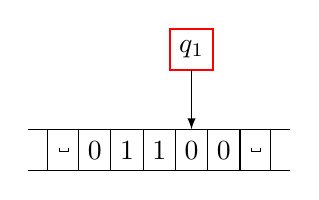
\begin{tikzpicture}[every node/.style={block}, block/.style={minimum height=1.5em,outer sep=0pt,draw,rectangle,node distance=0pt}]
            \node (C) {$1$};
            \node (B) [left=of C] {$1$};
            \node (A) [left=of B] {$0$};
            \node (0) [left=of A] {$\textvisiblespace$};
            \node (D) [right=of C] {$0$};
            \node (E) [right=of D] {$0$};
            \node (1) [right=of E] {$\textvisiblespace$};
            \node (F) [above = 0.75cm of D,draw=red,thick] {$q_1$};
            \draw[-latex] (F) -- (D);
            \draw (0.north west) -- ++(-.25cm,0) (0.south west) -- ++ (-.25cm,0) 
                (1.north east) -- ++(.25cm,0) (1.south east) -- ++ (.25cm,0);
        \end{tikzpicture}

        \vspace{20px}

        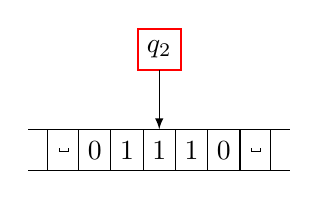
\begin{tikzpicture}[every node/.style={block}, block/.style={minimum height=1.5em,outer sep=0pt,draw,rectangle,node distance=0pt}]
            \node (C) {$1$};
            \node (B) [left=of C] {$1$};
            \node (A) [left=of B] {$0$};
            \node (0) [left=of A] {$\textvisiblespace$};
            \node (D) [right=of C] {$1$};
            \node (E) [right=of D] {$0$};
            \node (1) [right=of E] {$\textvisiblespace$};
            \node (F) [above = 0.75cm of C,draw=red,thick] {$q_2$};
            \draw[-latex] (F) -- (C);
            \draw (0.north west) -- ++(-.25cm,0) (0.south west) -- ++ (-.25cm,0) 
                (1.north east) -- ++(.25cm,0) (1.south east) -- ++ (.25cm,0);
        \end{tikzpicture}
        \hspace{20px}
        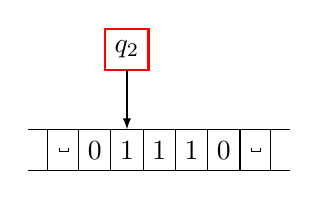
\begin{tikzpicture}[every node/.style={block}, block/.style={minimum height=1.5em,outer sep=0pt,draw,rectangle,node distance=0pt}]
            \node (C) {$1$};
            \node (B) [left=of C] {$1$};
            \node (A) [left=of B] {$0$};
            \node (0) [left=of A] {$\textvisiblespace$};
            \node (D) [right=of C] {$1$};
            \node (E) [right=of D] {$0$};
            \node (1) [right=of E] {$\textvisiblespace$};
            \node (F) [above = 0.75cm of B,draw=red,thick] {$q_2$};
            \draw[-latex] (F) -- (B);
            \draw (0.north west) -- ++(-.25cm,0) (0.south west) -- ++ (-.25cm,0) 
                (1.north east) -- ++(.25cm,0) (1.south east) -- ++ (.25cm,0);
        \end{tikzpicture}
        \hspace{20px}
        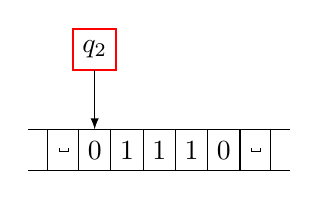
\begin{tikzpicture}[every node/.style={block}, block/.style={minimum height=1.5em,outer sep=0pt,draw,rectangle,node distance=0pt}]
            \node (C) {$1$};
            \node (B) [left=of C] {$1$};
            \node (A) [left=of B] {$0$};
            \node (0) [left=of A] {$\textvisiblespace$};
            \node (D) [right=of C] {$1$};
            \node (E) [right=of D] {$0$};
            \node (1) [right=of E] {$\textvisiblespace$};
            \node (F) [above = 0.75cm of A,draw=red,thick] {$q_2$};
            \draw[-latex] (F) -- (A);
            \draw (0.north west) -- ++(-.25cm,0) (0.south west) -- ++ (-.25cm,0) 
                (1.north east) -- ++(.25cm,0) (1.south east) -- ++ (.25cm,0);
        \end{tikzpicture}
        \hspace{20px}
        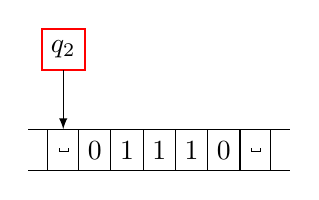
\begin{tikzpicture}[every node/.style={block}, block/.style={minimum height=1.5em,outer sep=0pt,draw,rectangle,node distance=0pt}]
            \node (C) {$1$};
            \node (B) [left=of C] {$1$};
            \node (A) [left=of B] {$0$};
            \node (0) [left=of A] {$\textvisiblespace$};
            \node (D) [right=of C] {$1$};
            \node (E) [right=of D] {$0$};
            \node (1) [right=of E] {$\textvisiblespace$};
            \node (F) [above = 0.75cm of 0,draw=red,thick] {$q_2$};
            \draw[-latex] (F) -- (0);
            \draw (0.north west) -- ++(-.25cm,0) (0.south west) -- ++ (-.25cm,0) 
                (1.north east) -- ++(.25cm,0) (1.south east) -- ++ (.25cm,0);
        \end{tikzpicture}
        
        \vspace{20px}

        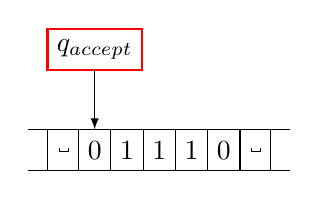
\begin{tikzpicture}[every node/.style={block}, block/.style={minimum height=1.5em,outer sep=0pt,draw,rectangle,node distance=0pt}]
            \node (C) {$1$};
            \node (B) [left=of C] {$1$};
            \node (A) [left=of B] {$0$};
            \node (0) [left=of A] {$\textvisiblespace$};
            \node (D) [right=of C] {$1$};
            \node (E) [right=of D] {$0$};
            \node (1) [right=of E] {$\textvisiblespace$};
            \node (F) [above = 0.75cm of A,draw=red,thick] {$q_{accept}$};
            \draw[-latex] (F) -- (A);
            \draw (0.north west) -- ++(-.25cm,0) (0.south west) -- ++ (-.25cm,0) 
                (1.north east) -- ++(.25cm,0) (1.south east) -- ++ (.25cm,0);
        \end{tikzpicture}
    \end{figure}

    \textbf{Part Two} What is the functionality of \(M\)? Justify your answer.
    \\

    Given a word that represents a number in binary, it will increment it by one based
    on the rules of binary addition.
    \\

    \textbf{Justification}
    \\

    In binary addition a 1 is added to the farthest right place value of
    the number. If this value is 1, it will flip it to 0 and carry to the next
    place value to the left.
    \\

    This flipping will occur until a 0 is reached or the read/write head reaches the end
    of the number. It will then flip the 0 to a 1, or the space to a 1.
    \\

    The result is that the binary representation of the number will be incremented by one.
\end{homeworkProblem}

\pagebreak

\begin{homeworkProblem}
    Let \(L\) be the language of \(\Sigma = \{0, 1\}\). Prove that \(L\)
    is Turing-decidable if and only if \(L\) can be enumerated by an enumerator
    Turing machine in strictly increasing order.

    \begin{proof}
        This proof will consist of two parts. First proving that any \(L\)
        that is Turing-decidable can be enumerated by an enumerator Turing machine
        in strictly increasing order. The second part is that an enumerator Turing machine
        in strictly increasing order gives a language, \(L\), that is Turing-decidable.
        \\

        \textbf{Part One}
        Proving that any Turing-decidable language can be enumerated by
        an enumerator Turing machine in strictly increasing order.
        \\

        This concludes the first part of the proof.
        \\

        \textbf{Part Two}
        Proving that any enumerator Turing machine in strictly increasing order
        gives a language, \(L\), that is Turing-decidable.
        \\


        This concludes the second part of the proof.
        \\

        Since both sides have been proven, the proof is complete.
    \end{proof}
\end{homeworkProblem}

\end{document}
